\chapter{Background}
\label{ch:background}

This chapter establishes the theoretical foundations and reviews the relevant literature to contextualise the later contents of this thesis. It begins by formally defining concept drift and outlining its taxonomy based on probabilistic decomposition and temporal characteristics. Subsequently, the general architecture of drift detection systems is analysed, alongside a review of some existing concept drift detectors and their inherent limitations. The chapter then moves on to consider a security perspective, introducing the notion of adversarial concept drift, where distributional shifts are manipulated by potentially malicious actors. Before turning to defences, it introduces the foundations of class-incremental learning and exemplar-based memory, which underpin how adaptive learners update without forgetting. Finally, the chapter concludes by discussing the already existing robust solutions, which have been proposed to mitigate these challenges.

\section{Concept Drift}
Concept drift generally refers to changes in the statistical relationship between input features and target labels, characterised as a change in the true joint distribution $p(X, y)$~\cite{Gao_2007}. Formally, concept drift between time points $t_0$ and $t_1$ is said to occur when
\begin{equation}
    p_{t_0}(X, y) \neq p_{t_1}(X, y),
\end{equation}
where $p_{t_0}$ and $p_{t_1}$ denote the joint distributions of the input variables $X$ and target variable $y$ at times $t_0$ and $t_1$, respectively~\cite{Gama_2014}.

\subsection{Taxonomy of Drift}
\subsubsection{Probabilistic Nature}
The joint probability can be given by the decomposition 
\begin{equation}
    p(X, y) = p(y \mid X)p(X)
\end{equation}
where $p(y \mid X)$ is the conditional distribution of the target given the input features and $p(X)$ is the probability distribution of the input features. Based on this, the literature~\cite{Gao_2007, Gama_2014, Korycki_2022} distinguishes between two forms of concept drift:

\begin{enumerate}
    \item \textit{Real drift}: When $p(y \mid X)$ changes without a change in $p(X)$ (Conditional Change) or with it (Dual Change). This is the more critical form of drift, as it directly affects decision rules or classification boundaries, making model adaptation necessary.
    
    \item \textit{Virtual drift (feature change)}: When $p(X)$ changes without affecting $p(y \mid X)$. While this may appear less important than real drift because the decision function is left unchanged, it cannot be ignored. In particular, changes in $p(X)$ may trigger adaptation or forgetting mechanisms, potentially leading to unnecessary or even harmful model updates.
\end{enumerate}

\subsubsection{Temporal Characteristics}
In addition to the above types, based on probabilities, concept drift can be categorised based on how the change occurs over time. Namely, four common patterns are shown in~\cref{fig:drift types}~\cite{Lu_2018}.

\begin{enumerate}
    \item \textit{Sudden/abrupt drift} is when the instance distribution or concept changes within a very short time frame. The previous concept immediately becomes invalid, and the learner must adapt quickly to maintain performance~\cite{Korycki_2022}.
    
    \item \textit{Gradual drift} is where instances from the old and new concepts coexist for a period, with old appearing with decreasing frequency~\cite{Korycki_2022}.
    
    \item \textit{Incremental drift} is when there is a smooth and continuous progression from one concept to another through a series of intermediate concepts~\cite{Gama_2014, Korycki_2022}.
    
    \item \textit{Reoccurring concepts} refers to when previously seen concepts reappear after some time, such as in seasonal or cyclical patterns~\cite{Gama_2014}. They may reappear either suddenly or incrementally~\cite{Guzy_2020}.
\end{enumerate}

\begin{figure}[h]
    \centering
    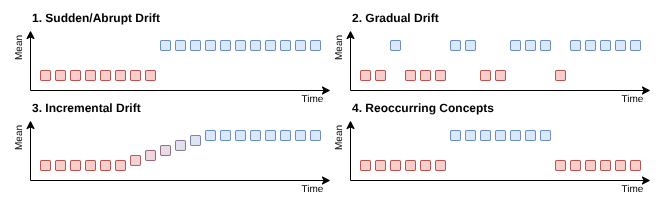
\includegraphics[width=\linewidth]{background/drift types.drawio.png}
    \caption{Examples of concept drift types based on temporal patterns}
    \label{fig:drift types}
\end{figure}


\section{Concept Drift Detection}
\label{sec:drift_detection}
In data stream learning, concept drift is typically addressed by augmenting the predictive model (the base learner) with a drift detection mechanism. In general, drift detectors attempt to identify changes in the data distribution by analysing the base learner's behaviour~\cite{Barros_2018}. Rather than continuously retraining the learner, drift detectors act as a supervisory mechanism, triggering an adaptation process, such as model retraining, parameter update, or selective forgetting of historical data.

\subsection{General Architecture of Drift Detection Systems}
\label{sec:drift detection architecture}
Although they are algorithmically diverse, most concept drift detection systems follow a common architectural pattern. This architecture can be decomposed into four conceptual components:

\begin{enumerate}
    \item \textit{Observation source}: The detector monitors a stream of signals derived either from the data itself or from the performance of a base learner. Common sources include error rates, loss values, feature statistics, or latent representations.
    
    \item \textit{Summary mechanism}: Observations are aggregated over time using sliding windows, cumulative statistics, or incremental estimators. This step compresses the raw stream into a tractable representation that reflects the system behaviour of a given period.
    
    \item \textit{Change test}: A statistical test, threshold comparison, or learned decision rule evaluates whether the observed summary deviates significantly from a reference/historical summary. This comparison may rely on bounds derived from concentration inequalities, hypothesis tests, or reconstruction error metrics.
    
    \item \textit{Decision and response}: Upon detecting significant deviation, the detector emits a signal (sometimes distinguishing between a warning and confirmed drift) which triggers downstream actions such as retraining, window resetting, or model replacement.
\end{enumerate}

This modular structure highlights an important property of drift detectors: they act as \emph{control mechanisms} governing when and how adaptive learning occurs. As such, their behaviour has long-term consequences for system performance, stability, and robustness.

\subsection{Drift Detection Algorithms}
While the general architecture remains consistent, specific implementations differ in their observation sources and statistical tests. The literature typically categorises these methods into error rate-based and data distribution-based approaches~\cite{Lu_2018}.

\subsubsection{Error Rate-Based Detectors}
These methods monitor the online performance of the base learner (e.g. classification accuracy). They function based on the assumption that a statistically significant increase or decrease in model performance implies a change in the underlying data distribution~\cite{Lu_2018}. Drift detectors in this category include:

\begin{itemize}
    \item \textit{Drift Detection Method (DDM)}~\cite{Gama_2004}: This method models the number of errors as a random variable from a Binomial distribution. It tracks the online error rate $p_t$ and its standard deviation $s_t = \sqrt{p_t(1-p_t)/t}$ at time $t$. The algorithm maintains the minimum values observed so far, $p_{min}$ and $s_{min}$, updating them whenever $p_t + s_t < p_{min} + s_{min}$. A warning level is triggered if: 
    \begin{equation} \label{eq:DDM warning}
        p_t + s_t \geq p_{min} + 2s_{min},
    \end{equation}
    at which point incoming examples are buffered while using the old learner for predictions. If the error rate continues to rise and drift is confirmed via the condition: 
    \begin{equation} \label{eq:DDM confirmation}
        p_t + s_t \geq p_{min} + 3s_{min},
    \end{equation}
    a new learner is induced using the buffered examples, and the old learner is discarded.
    % DDM is effective for detecting abrupt drift but can be less sensitive to gradual changes or noisy data streams.

    \item \textit{ADaptive WINdowing (ADWIN)}~\cite{Bifet_2007}: This method uses a sliding window $W$ that dynamically adjusts its size, based on the rate of change in the data stream. It operates by examining all possible cuts of the current window into two sub-windows, $W_{0}$ and $W_{1}$, representing historical and newer data, respectively. Drift is detected if the absolute difference between the averages of these sub-windows is statistically significant:
    \begin{equation} \label{eq:ADWIN threshold}
        |\hat{\mu}_{W_0} - \hat{\mu}_{W_1}| \geq \epsilon_{cut}
    \end{equation}
    where $\epsilon_{cut}$ is an adaptive threshold (determined using Hoeffding bounds and a confidence interval $\delta$). When this threshold is reached, the historical data ($W_{0}$) is discarded as the two sub-windows are seen to have come from different data distributions. The author's also proved that the false positive and false negative rates are bounded by $\delta$.
\end{itemize}

\subsubsection{Data Distribution-Based Detectors}
In contrast, these methods monitor the statistical properties of the input features ($P(X)$), independent of the base learner's behaviour and error rate. They rely on the assumption that drift can be signalled by a statistically significant deviation in the distribution of new data when compared to a historical reference window~\cite{Lu_2018}. Because they analyse the input data itself, these methods can detect virtual drift that does not immediately alter the decision boundary and can also function when ground truth labels are unavailable. Examples of data distribution-based detectors include:

\begin{itemize}
    \item \textit{Statistical Change Detection for multidimensional data (SCD)}~\cite{Song_2007}: This detector addresses the challenge of multidimensional distribution change by employing a non-parametric statistical test known as the Density Test. The baseline/historical window $S$ is partitioned into two halves: $S_1$ for modelling and $S_2$ for testing. It utilises a Kernel Density Estimator (KDE) on $S_1$, to get the density function $\mathscr{K}_{S_1}$. The test statistic $\delta$ is then defined using the difference in log-probability density of $\mathscr{K}_{S_1}$ at $S'$ and at $S_2$. Specifically:
    \begin{equation}
        \delta = LLH(\mathscr{K}_{S_1}, S') - \frac{|S'|}{|S_2|} \times LLH(\mathscr{K}_{S_1}, S_2)
    \end{equation}
    where $LLH$ is the log-likelihood. Drift is confirmed if $\delta$ falls below a critical value $C_{max}$ (algorithmically derived from a user-defined significance level $p$).

    \item \textit{Principal Component Analysis-Based Change Detection (PCA-CD)}~\cite{Qahtan_2015}: This method works on multidimensional data streams by projecting the data onto lower-dimensional spaces using PCA. It extracts the top $k$ principal components that explain a substantial portion of the variance from the historical window and then monitors new data projected onto these components as separate univariate streams. Similarly to SCD, the density of these projections is estimated using KDE, for example. A divergence metric, such as the intersection area under the curves of the reference ($\hat{f}$) and test ($\hat{g}$) distributions:
    \begin{equation}
        D_{A}\left(\hat{g}\,||\,\hat{f}\right) = 1 - \int_{x} \min\left(\hat{f}(x), \hat{g}(x)\right) dx
    \end{equation}
    is calculated for each of the $k$ components. Then the final change score is taken as the maximum of these. To detect drift, the method applies the Page-Hinkley (PH) test with a dynamic threshold to the aggregate score, triggering an alarm when the cumulative deviation from the historical mean exceeds a given limit.
\end{itemize}

\subsection{Limitations and Weaknesses}
While the drift detectors described above do provide robust mechanisms for adaptation, they are subject to inherent limitations and trade-offs between sensitivity (minimising false negatives) and specificity (minimising false positives). Rather than arising from flawed algorithms, many of these weaknesses are due to the statistical assumptions made by classical drift detection; most notably, finite-sample estimation, approximate stationarity within windows, and the use of fixed confidence bounds to identify change.

These limitations can be mapped onto the general architecture of drift detectors introduced earlier in~\cref{sec:drift detection architecture}. Choices made at the level of the observation source (e.g. error rates or feature statistics), the summary mechanism (e.g. windowing or cumulative statistics), and the change test (e.g. hypothesis tests or thresholds) impose constraints on what types of drift can be reliably identified and how quickly.

\subsubsection{Sensitivity to Gradual Drift}
A limitation of some error-based detectors, such as DDM, is the reduced ability to distinguish between stationary noise and gradual concept drift. In the presence of abrupt drift, the error rate typically exhibits a sharp increase, triggering the detector's thresholds (defined for DDM in~\cref{eq:DDM warning} and~\cref{eq:DDM confirmation}). However, during a gradual drift, the error rate may increase too slowly to violate the statistical bounds.

Under such conditions, the detector may update its internal reference statistics ($p_{min}$ and $s_{min}$ in the case of DDM), effectively incorporating the drifted distribution into its baseline instead of identifying it. While adaptive windowing approaches, such as ADWIN, mitigate this by dynamically adjusting the window size, they are still bounded by the resolution of their sliding window. Drift, which remains below the statistical bound (defined for ADWIN as $\epsilon_{cut}$ in~\cref{eq:ADWIN threshold}), will remain undetected until enough samples accumulate to reach statistical significance.

Fundamentally, this limitation highlights the difficulty in distinguishing between slow drift and stationary noise under bounded confidence levels, without making additional assumptions about the drift process. Any attempt to increase sensitivity by lowering detection thresholds inevitably raises the false positive rate, highlighting a trade-off key to all hypothesis test-based or threshold-based drift detectors.

\subsubsection{Verification Latency and Label Availability}
Error-based detectors suffer from a critical dependency on ground truth availability. They assume that labels are available immediately or with minimal delay after the prediction is made, to compute prediction errors and monitor performance degradation. In many real-world streaming applications, such as credit fraud detection or loan forecasting, the true label may arrive with significant delay (verification latency) or may never arrive at all. 

During periods of high verification latency, the detector effectively cannot observe its primary signal, leaving the system blind to changes in performance. If drift occurs during such a period, the system will continue to trust an outdated model, accumulating loss until detection becomes possible.

\subsubsection{Virtual Drift and False Positives}
Distribution-based detectors address the problem with label dependency by monitoring the input feature distribution $P(X)$ rather than model error. While this enables detection in settings with delayed or missing labels, it introduces a different weakness related to virtual drift. A statistically significant change in $P(X)$ does not always imply a change in the conditional distribution $P(y \mid X)$. It therefore does not guarantee that the predictive decision boundary has changed.

Consequently, distribution-based detectors may generate false positives, triggering model retraining or data forgetting even when performance remains stable (there is no real drift). Such unnecessary adaptation can be computationally expensive and may temporarily degrade performance.

\subsubsection{Dimensionality and Feature Relevance}
In high-dimensional settings, distribution-based detectors rely on density estimation or projection techniques that are sensitive to the curse of dimensionality. As the number of dimensions increases, data sparsity reduces the reliability of density estimates, while dimensionality reduction risks discarding directions along which drift is relevant. Moreover, distribution-based detectors typically treat all features with equal importance, meaning they are susceptible to changes in weakly relevant features that may not materially affect model performance.


\section{Adversarial Concept Drift}
Classical concept drift assumes that changes in the data distribution arise from natural, exogenous factors such as evolving user behaviour, seasonality, or changes in the underlying environment. In contrast, adversarial drift assumes that there is a purposeful and potentially malicious actor attempting to manipulate our adaptive learning system~\cite{Korycki_2022}. The potential goals they may have will be discussed in the next section. 

In such settings, the drift process is no longer passive. Instead, the data stream itself becomes an attack surface, and the drift detector becomes a target. Adversarial drift extends traditional data poisoning attacks by exploiting temporal dynamics and specific detector behaviours. Rather than corrupting a static training set, the adversary seeks to control when adaptation is triggered, what data is included during retraining, and which information is forgotten. This introduces a new class of threats that cannot be fully explained by classical adversarial learning models alone~\cite{Kloft_2010}.

\subsection{Adversarial Objectives}
An adversary interacting with an adaptive learning system may pursue several objectives, which are not mutually exclusive.

A primary objective could be \emph{performance degradation}, where the adversary seeks to reduce the predictive accuracy or increase the loss of a system~\cite{Sethi_2018}. Unlike poisoning attacks, adversarial drift may be gradual, ensuring that degradation accumulates slowly while remaining below detection thresholds.

This could be seen as a potential secondary objective: \emph{evasion of detection}. Here, the adversary aims to avoid the activation of the drift detector while pursuing their primary objective. This could involve crafting inputs that move the decision boundary while preserving the statistics monitored, hence exploiting the blind spots of classical detectors.

Alternatively, an adversary may attempt \emph{forced adaptation}, deliberately triggering false drift alarms to cause unnecessary retraining or forgetting. Such behaviour can destabilise the learning process, increase computational costs, or induce catastrophic forgetting of valid historical concepts~\cite{Korycki_2022}. Conversely, an adversary could seek to \emph{block adaptation}, injecting contradictory data points during a period of valid concept drift, in an attempt to nullify the adaptation process~\cite{Korycki_2022}.

Finally, adversaries may seek \emph{control over the learned concept}, gradually forcing the system to learn a decision boundary favourable to the attacker’s goals. In this case, the detector is actively exploited as a mechanism for injecting the poisoned instances during adaptation cycles.

\subsection{Instance-Based Poisoning}
Instance-based poisoning attacks are those in which an adversary injects or modifies individual data points in the stream to influence the base learner or drift detector. These attacks are powerful because the poisoned instances can be distributed over time, allowing adversaries to exploit both the learner’s update behaviours and the detector’s temporal assumptions. For example, poisoned samples may be injected intermittently or gradually, ensuring that individual instances appear benign while the cumulative effect leads to performance degradation or detector manipulation.

From a drift detection perspective, instance-based poisoning can be used to:
\begin{itemize}
    \item \textit{Bias summary statistics}: By subtly increasing error rates or similar statistics within certain bounds, the adversary can influence the detector's inner mechanisms.
    \item \textit{Trigger false alarms}: Bursts of or extreme poisoned instances may surpass thresholds, triggering unnecessary adaptation or window resets.
    \item \textit{Suppress true drift detection}: Conversely, carefully engineered samples can stabilise monitored statistics during periods of genuine drift, delaying or preventing detection~\cite{Korycki_2022}.
\end{itemize}

Crucially, even small, strategically placed perturbations can be sufficient to accumulate and have the desired effect, particularly against detectors based on hypothesis testing or confidence bounds. This makes instance-based poisoning difficult to distinguish from natural noise or gradual drift, especially in high-variance data streams.

% While many drift detectors incorporate safeguards such as conservative thresholds, ensemble monitoring, or robust statistics, these defences are designed under the assumption of stochastic rather than adversarial data generation. As a result, they may remain vulnerable to coordinated instance-level attacks that exploit their reliance on finite-sample estimates and bounded confidence levels.

\subsection{Concept-Based Poisoning}
Concept-based attacks function at a higher level of abstraction than instance-based attacks. Rather than focusing on individual samples, the adversary aims to directly mimic a shift in the data-generating process to falsify genuine concept drift. The adversary engineers the drift trajectory to achieve a desired outcome, such as the misclassification of specific regions of the input space or the biased treatment of certain inputs.

By anticipating how the detector responds to changes in monitored statistics, the adversary can:
\begin{itemize}
    \item \textit{False adaptation}: Triggering adaptation where the system interprets the adversarial concept as a genuine distributional change~\cite{Korycki_2022}.
    \item \textit{Exploit forgetting mechanisms}: Causing the system to discard historically valid or important data.
    \item \textit{Suppressed adaptation}: Balancing genuine concept drift with a conflicting distribution, preventing the detector from reaching its change threshold or negatively impacting the adaptation process.
\end{itemize}

% Such attacks are particularly effective against detectors designed to respond to gradual or incremental drift. By aligning the induced change with expected temporal patterns, the adversary can ensure that adaptation mechanisms are triggered naturally, causing the learner to internalise a corrupted concept as if it were benign~\cite{Koh_2021}.


\section{Class-Incremental Learning and Exemplar Memory}
\label{sec:exemplar memory}
The drift detectors described so far are concerned with deciding when to adapt. Equally important is how a model is updated once said adaptation is triggered. When a learner is only retrained on newly arrived data, it can overwrite previously learned knowledge, a phenomenon known as catastrophic forgetting~\cite{French_1999}. This is especially problematic in streaming settings where reoccurring concepts are common and may reappear after the model has specialised to more recent traffic.

A common countermeasure is rehearsal (or replay), where a small memory of representative past examples, called exemplars, is retained and used alongside new data during each update~\cite{Robins_1995}. Given a finite memory budget, an important question is which examples to keep so the retained subset remains faithful to the data it summarises.

A widely adopted solution is the iCaRL (Incremental Classifier and Representation Learning) mechanism introduced by Rebuffi et al.~\cite{Rebuffi_2017}, which classifies using a nearest-mean-of-exemplars rule. Given a class with feature embedding $\phi(\cdot)$ and true mean
\begin{equation}
    \mu = \frac{1}{n}\sum_{x} \phi(x),
\end{equation}
herding greedily builds an ordered exemplar set $\{p_1, \dots, p_m\}$ of target size $m$, selecting the $k^{\text{th}}$ exemplar as the sample that brings the running exemplar mean closest to $\mu$:
\begin{equation} \label{eq:herding}
    p_k = \arg\min_{x} \left\| \mu - \frac{1}{k}\left( \phi(x) + \sum_{j=1}^{k-1} \phi(p_j) \right) \right\|.
\end{equation}
Because each successive exemplar maximally reduces the difference between the stored mean and the true class mean, any prefix of the resulting set remains representative of the class centroid, and the budget $m$ can be adjusted without re-selecting from scratch.

This property is particularly valuable for nearest-mean classifiers operating under bounded memory. Since the class prototype is computed from the stored exemplars rather than the full data history, a herded memory preserves the representation of that prototype while bounding both storage and retraining cost. This makes it a natural memory-management policy for an NCM-based drift detector that must register newly discovered concepts and retain a limited, representative sample of each for future retraining, a point we return to when describing the drift detector adopted in this thesis (\cref{sec:contrastive_ncm}).


\section{Adversarially Robust Solutions}
\label{sec:robust solutions}
To address the vulnerabilities of traditional detectors, recent research proposes methods explicitly designed to withstand adversarial manipulation. These solutions employ techniques like contrastive embedding and generative modelling to differentiate between natural and adversarial distributional shifts.

\subsection{Robust Restricted Boltzmann Machine for Drift Detection}
\label{sec:rrbm-dd}
Korycki and Krawczyk~\cite{Korycki_2022} introduce the Robust Restricted Boltzmann Machine for Drift Detection (RRBM-DD), a generative neural network that detects drift by monitoring the reconstruction error of incoming samples against a learned model of the past data distribution. That is, the RRBM encodes the recent distribution directly in its weights and the detector treats any sample that the model fails to reconstruct accurately as evidence of distributional change. The architecture also incorporates two distinct mechanisms designed to remain robust when the incoming stream is adversarially manipulated rather than naturally drifting.

To counter instance-based poisoning, the model is trained with a robust gradient descent procedure using M-estimators that softly truncate the influence of samples whose loss exceeds a learned tolerance. To counter concept-based poisoning, the model's energy function is augmented with a gating mechanism over the hidden layer and a Gaussian noise model over the visible layer. The gating allows individual hidden units to be deactivated when their contribution is dominated by an adversarial cluster, and the noise model damps reconstruction-error spikes caused by adversarial perturbations.

Korycki and Krawczyk evaluate the RRBM-DD as part of a coupled adaptive system where the downstream base learner is updated continuously. They employ an adaptive Hoeffding tree that incrementally revises its splits with each new labelled sample, independently of any drift signal. In this configuration, the detector's role is advisory: it can declare that drift has occurred, causing a full retraining, but the model still adapts continuously and so does not depend entirely on the detector to trigger updates. This contrasts with the setting examined in this thesis, in which a static base learner updates only when explicitly triggered by the detector and therefore inherits both the detector's robustness properties and its decision latency. The implications of this difference for adversarial robustness are taken up in~\cref{ch:target_system_threat_model}.

\subsection{The Contrastive NCM Detector}
\label{sec:contrastive_ncm}
% Kuppa and Le-Khac~\cite{Kuppa_2022} propose a detector that maps high-dimensional inputs to a low-dimensional latent space using a contrastive loss objective. To create tighter class clusters, which are naturally more robust to adversarial perturbations, this objective places similar samples closer together while spreading dissimilar ones apart.

Kuppa and Le-Khac~\cite{Kuppa_2022} introduce the Contrastive NCM detector, composed of three key components. A contrastive autoencoder which maps each raw input vector into a lower dimensional latent space where same-class samples cluster tightly. A Nearest Class Mean (NCM) classifier which uses a hybrid Euclidean-Riemannian distance metric to decide whether the incoming sample is consistent with one of the known classes or should be flagged as drifted. Finally, a recursive concept-discovery mechanism which accumulates drifted embeddings over time and, once a threshold is exceeded, registers a new class prototype or concept. This combination is designed to remain robust under adversarial inputs by combining the manifold-tightening effect of contrastive training with a distance metric that distinguishes adversarial samples from genuine novel ones.

\subsubsection{Contrastive Autoencoder}
The encoder $h : \mathbb{R}^d \to \mathbb{R}^r$ maps each $d$-dimensional input $x$ to a lower-dimensional latent embedding $h(x)$ (with $r < d$); we write $h_i = h(x_i)$ for the embedding of sample $x_i$. The autoencoder is trained jointly under two losses. The first is the standard mean-squared reconstruction loss
\begin{equation} \label{eq:ncm-mse}
    \mathcal{L}_{\text{MSE}} = \| g(h(x)) - x \|^2_2,
\end{equation}
where $g(\cdot)$ is the decoder. The second is a supervised contrastive term which aims to make the positive pairs attracted and the negative samples separated
\begin{equation} \label{eq:ncm-contrastive}
    \mathcal{L}_{\text{contrastive}} = - \sum_{i=1}^B \log \left[\frac{e^{s(h_i, v_k)}}{\sum_{j}^P e^{s(h_i, v_j)}}\right],
\end{equation}
where for a sample $x_i$ with embedding $h_i$ in class $k$, $v_k$ is the prototype of class $k$ in the latent space, $P$ is the number of known classes, $B$ is the batch size, and the similarity score
\begin{equation}
    s(h_i, v_j) = \frac{h_i^\top v_j}{\|h_i\| \|v_j\|} \cdot \frac{1}{\tau}
\end{equation}
is a temperature-scaled cosine similarity with temperature $\tau$. Class prototypes $v_k$ are computed as the mean embedding of samples in the batch belonging to class $k$. The combined objective $\mathcal{L} = \mathcal{L}_{\text{MSE}} + \mathcal{L}_{\text{contrastive}}$ encourages the encoder to produce a latent space that simultaneously preserves enough information to reconstruct the input (via $\mathcal{L}_{\text{MSE}}$) and clusters same-class samples tightly while pushing different-class samples apart (via $\mathcal{L}_{\text{contrastive}}$).

\subsubsection{Nearest Class Mean Classifier with Hybrid Distance}
Once the embedding network is trained, it is used to fit a Nearest Class Mean (NCM) classifier~\cite{Kuppa_2022} that decides which known class an incoming sample belongs to or whether it should be flagged as drifted. NCM is a distance-based classifier that assigns each incoming sample to the class with the closest prototype, here in latent space. Its accuracy depends critically on the choice of distance metric. For each known class $c$, the prototype is computed as the mean of the embeddings of its training samples:
\begin{equation} \label{eq:ncm-prototype}
    \bm{h}_c = \frac{1}{n_c} \sum_{i}\left[y_i=c\right] \mathbf{h}_i,
\end{equation}
where $n_c$ is the number of training samples observed for class $c$; this $\bm{h}_c$ is the full-data counterpart of the per-batch prototype $v_k$ in~\cref{eq:ncm-contrastive}, both being the latent-space centroid of a class. The assigned class for an incoming sample with embedding $\mathbf{h}_j$ is the one minimising a hybrid distance,
\begin{align}
    c_j^* &= \underset{c\in C}{\arg\min}\,D(\mathbf{h}_j, \bm{h}_c), \label{eq:ncm-classification}\\
    D(\mathbf{h}_j, \bm{h}_c) &= d_R(\mathbf{h}_j, \bm{h}_c) + \lambda_1(d_E(\mathbf{h}_j, \bm{h}_c)), \label{eq:hybrid-distance}
\end{align}
where $d_E$ is the Euclidean distance between the sample and the class prototype in latent space, $d_R$ is a Riemannian divergence (geometric distance) between them, $\lambda_1 > 0$ is a tuning parameter controlling their relative contribution, and $C$ is the set of known class indices.

The two terms in the metric are intended to capture both instance and group level fidelity. The Euclidean term enforces instance level fidelity, while the Riemannian term enforces group level fidelity. Their combination is claimed to be robust against adversarially-crafted inputs by exploiting three properties of adversarial subspaces~\cite{Kuppa_2022}: (a) they are found in lower-probability regions compared to the data manifold; (b) their class distributions tend to vary from their closest natural sub-manifold; and (c) an adversarial sample's nearest neighbour is its unperturbed source, rather than any other point in the training or test set.

The same hybrid distance is also used to identify drifted samples. A sample is taken as evidence of a previously unobserved class when its distance to the nearest known prototype is large. Concretely, a sample $x_j$ with embedding $\mathbf{h}_j$ is flagged as drifted when its minimum hybrid distance to the known prototypes exceeds a drift threshold $T_{drift}$,
\begin{equation} \label{eq:drift-rule}
    \min_{c \in C} D(\mathbf{h}_j, \bm{h}_c) > T_{drift},
\end{equation}
where $D$ is the hybrid distance of~\cref{eq:hybrid-distance} and $C$ is the set of known class indices. Kuppa and Le-Khac~\cite{Kuppa_2022} do not formally specify how $T_{drift}$ should be derived. We describe the calibration procedure adopted in this thesis in~\cref{ch:implementation}.

\subsubsection{Concept Discovery}
\label{sec:concept_discovery}
Drifted samples alone do not invalidate the model; instead, the detector treats them as candidate evidence of a new class. Drifted embeddings $\{\mathbf{z}_{1_{drift}}^t, \mathbf{z}_{2_{drift}}^t, \dots\}$ produced during a time window $t$ are buffered, and the detector maintains a running accumulator
\begin{align} \label{eq:concept-accumulator}
    \Delta_{drift}^{t \to t+1} &= \bm{h}_c^{t+1} - \bm{h}_c^t = \Delta^{t-1 \to t} + \delta^{t-1 \to t},\\
    \delta_i^{t-1 \to t} &= \mathbf{z}_{i_{drift}}^t - \mathbf{z}_{i_{drift}}^{t-1}\: y_i\in c^t.
\end{align}
Intuitively, $\delta_i^{t-1 \to t}$ is the displacement of each drifted embedding between successive windows, and $\Delta_{drift}$ accumulates these displacements over time. Once the resulting magnitude is large enough, the buffered samples are taken to form a coherent new concept. When the accumulated displacement crosses a threshold $T$,
\begin{equation} \label{eq:concept-threshold}
    \|\Delta_{drift}^{t \to t+1}\| > T,
\end{equation}
new mean class prototypes $h_{new,i}$ are registered, both the accumulator and buffer are reset, and the autoencoder is retrained on new data that includes the newly identified class. The paper does not specify how past concepts in the dataset are maintained under bounded memory across retraining cycles. A natural choice, following the rehearsal principles in~\cref{sec:exemplar memory}, is to represent each registered class by a fixed-size exemplar set selected via herding (\cref{eq:herding}); we adopt this in~\cref{ch:implementation}.

\subsubsection{Operational Protocol}
The detector therefore both decides when adaptation is required (via the drift threshold $T_{drift}$ and the concept discovery threshold $T$) and identifies which incoming samples were candidate evidence for that adaptation (via the concept-discovery buffer). What is not specified by Kuppa and Le-Khac~\cite{Kuppa_2022} is how this adaptation interacts with any downstream classifier, nor how the candidate evidence should be combined with retained known-class data when the encoder is retrained. We return to these architectural questions in~\cref{ch:target_system_threat_model,ch:implementation}.
